\chapter{Introduction}
\label{chap:intro}


\section{Introduction}
%{\bf Below is a bullet list of items that should be discussed in the introduction}
%\begin{itemize}
%\item Basic discussion of LIGO, gravitational wave sources, numerical simulations.
%\item Discussion of two-body problem in GR (black holes and neutron stars).
%\item How are BNS binaries formed? What is known astrophysically?
%\item  In this thesis we discussion binaries with a spinning NS....
%\item Discussion of IVP in GR (matter and non-matter). Junk radiation?
%\item Discussion of contemporary BNS sims. What is being done?
%\item What is in the thesis?
%\end{itemize}

September 14th, 2015 marked the dawning of a new age in astronomy -- the age of gravitational wave astronomy. The extraordinary detection of merging black holes by Advanced LIGO~\citep{LIGOVirgo2016a} left no doubt of this. After a second detection of merging black holes on December 26th, 2015,~\cite{Abbott:2016nmj}, we are left anxiously waiting what will be in store for us next. The first detection was made just before Einstein's theory of general relativity (GR)~\citep{Einstein:1915by} turned one hundred years old. Indeed, one of its most striking predictions is the existence of gravitationl waves (GWs) - ripples in space-time that propagate at the speed of light. One of the ways these gravitational waves are generated is through the inspiral of compact object binaries. In these binaries, a neutron star (NS) or a black hole (BH), orbits with a NS/BH companion about their common centre of mass. Over time, through the emission of GW, the orbit shrinks and eventually the objects merge. Previously, these GW have never been directly detected, although their existence had been indirectly confirmed. Hulse and Taylor won the 1993 Nobel Prize for their observations of the Hulse-Taylor pulsar~\citep{Hulse:1974eb} - a binary pulsar system whose orbital decay was carefully measured and found to match perfectly with the predctions of general relativity. Further observations have since strengthened these findings; see \cite{Berti:2015itd} for a detailed review of current and future tests of GR. 

Ground-based interferometric gravitational wave detectors are poised to make many more direction detections of GWs. With Advanced LIGO~\citep{aLIGO1,aLIGO2} already doing so, and Advanced Virgo ~\citep{AdV,TheVirgo:2014hva} and KAGRA~\cite{Somiya:2012}) coming on soon, a wealth of results awaits. Advanced LIGO expects a realistic event rate $\sim 30$ binary neutron star mergers per year at design sensitivity, with a horzion diestance of $\sim 200$ Mpc. Similarly, an event rate of $\sim 10$ mergers per year is expected for binary black holes, and $\sim 10$ for BH-NS binaries. These detectors are sensitive to frequencies of $\sim 10{\rm Hz} - 1{\rm kHz}$. Other detection methods, like pulsar timing arrays~\citep{Joshi:2013at}, are sensitive to very different frequency bands ($300{\rm pHz}-100{\rm nHz}$).

These ground-based detectors use the technique of matched filtering~\citep{Owen:1998dk} to make detections, in which the observed signal is mathced against template waveforms to search for the astrophysical signal. These templates are generated either analytically, using, for example, Post-Newtonian (PN) theory, a perturbative expansion of GR, or by using numerical relativity (NR), in which the Einstein Field Equations are solved numerically on sumpercomputers. PN waveforms are computationally cheap to produce but become increasingly inaccurate near merger, while NR waveforms are more accurate, but are costly to produce. Hybridization techniques~\citep{MacDonald:2012mp} ``stitch'' PN waveforms together with NR waveforms to get the best of both worlds.

The parameter space of numerical relativity simulations of black hole binaries is seven dimensional. Each black hole has a spin vector $\vec{\chi}$ with three components, and their mass ration $q\equiv m_1/m_2$, where $m_1$ is the mass of the larger hole, is the 7th dimension. The total mass of the binary is scaled out of the numerical problem. Most compact object systems are expected to circularize~\citep{PetersMathews1963,Peters1964} in their orbits before merger, so we do not regard orbital eccentriccity as part of the parameter space. Spanning this parameter space is a difficult endeavour for numerical relativity collaborations and much of it remains uncovered~\citep{Mroue:2013PRL,Chu:2015kft}. Various dimensional reduction technqiues~\citep{Canizares:2014fya} are used for Advanced LIGO template banks. Once matter is added to simulations, through neutron stars, the parameter space increases signficantly. In addition to the seven parameters already present in the black hole binaries, the total mass of the system is now a parameter, as the maximum NS provides a natural phsyical mass scale. This can affect, for example, whether or not a hyper-massive neutron star is present after the merger of binary neutron stars or if direct collapse to a black hole occurs. In addition, the NS equation of state (EOS) becomes important to the system. Since the equation of state of dense nuclear matter is not currently known, constrainting the NS EOS from gravitational wave observations is an important goal of advanced ground-based detectors. Additionally, once a neutron star is present, simulations can study additional physics such as neutrino transport, nuclear reactions, and magnetic fields. Such ingredients are crucial for understand the electromagnetic emission likely to come from a BNS or BHNS merger.

BNS binaries, unlike BBH and BHNS bianries, have been observed and studied within our galaxy, and therefore the expections of Advanced LIGO for NSNS binaries are more tightly constrained. The known binary neutron star population is summarized in table~\ref{tab:BNSPop}~\citep{Postnov:2014tza}. We report the spin periods, orbital periods, eccentricites, characteristic life-times ($\tau_{c}=\dot{P}/2P$), time until merger, and the final spin periods of systems that will merge in a Hubble time. The system J0737-3039 is particuarly interesting, as one fot the NSs will merge with a spin period of 22.4ms. This is comparable enough to the orbtial timescale near merger, $P\sim 2ms$, to be relevant to GW data analysis. NSs in binaries are spinning, and thus it is important to do NR simulations of spinning BNS binaries. For many years, spin was a largely unexamined dimension of the BNS paramter space, although there has been a significant interest lately. Note, however, that the spins would have to be innate, since neutron star viscosity is not nearly large enough for tidal torques to be effective in spinning the stars up~\citep{BildstenCutler1992}.

 
 \begin{table}
\centering
 \caption{The properties of known double neutron star systems.}
\label{tab:BNSPop}
 \begin{tabular}{c || c | c | c | c | c | c}
%\label{tab:BNSPop}
 \hline
 System & $P(ms)$ & $P_{\textnormal{orb}}(d)$ & $e$ & $\log_{10}{\tau_c(yr)}$ & $\log_{10}{\tau_g(yr)}$ & $P_f(ms)$ \\
 \hline \hline
 J0737-3039 & 22.7 & 0.102 & 0.088 & 8.3 & 7.9 & 26.8 \\
 J0737-3039 &  2770 & 0.102 & 0.088 & 7.7 & 7.9 &   4453 \\
 J1518+4904 & 40.9 & 8.6 & 0.25 & 10.3 & 12.4 & --- \\
 B1534+12 & 37.9 & 0.32 & 0.27 & 8.4 & 9.4 & 126 \\
 J1756-2251 & 28.5 & 0.32 & 0.18 & 8.6 & 10.2 & --- \\
 J1811-1736 & 104.2 & 18.8 & 0.83 & 9.0 & 13.0 & --- \\
 B1820-11 & 279.8 & 357.8 & 0.79 & 6.5 & 15.8 & --- \\
 J1829+2456 & 41.0 & 1.18 & 0.14 & 10.1 & 10.8 & --- \\
 J1906+0746 & 144.1 & 0.17 & 0.085 & 5.1 & 8.5 & 7224 \\
 B1913+16 & 59.0 & 0.3 & 0.62 & 8.0 & 8.5 & 120 \\
 B2127+11C & 30.5 & 0.3 & 0.67 & 8.0 & 8.3 & 52.6 \\ 
 \end{tabular}
 \end{table}
 

This thesis is largely interested in spining neutron stars in numerical relativity. The structure is as follows: In chapter~\ref{chap:bns}, we discuss our work on initial data and evolutions of spinning BNS binaries using the SpEC code. In chapter~\ref{chap:bhns}, we disucss the exntension of this initial data formalism to BHNS binaries with a spinning NS. In chapter~\ref{chap:jr}, we shift focus and discuss work we have done on understanding the nature of spurious gravitational radiation, commonly known as ``junk radiation'', in BBH systems. Finally, in chapter~\ref{chap:conc} we conclude and summarize the thesis and discuss future possibilities.

The remainder of this introduction is structured as follows: In Section~\ref{sec:TwoBody} we review the 2-body problem in GR and discuss some basic Post-Newtonian theory. In section~\ref{sec:IVP}, we review the initial value problem in NR. Finally, in section~\ref{sec:BNS} we discuss some basic astrophysical properties of binary neutron star systems and black hole--neutron star systems.

%{\bf Below is a copy-paste of the introduction of my thesis proposal. This must be updated}

%Einstein's theory of general relativity predicts that gravitational waves will be generated by strong gravitational events. Although so far these gravitational waves have only been detected indirectly (e.g., though the orbital decay of the Hulse-Taylor pulsar), detectors like the Laser Interferometer Gravitational Wave Observatory (LIGO) and VIRGO now have the capability, in principle, to detect gravitational waves. The expected events rates for the initial detectors were only on the order of a few per century
%so it is not surprising that there have been no detections so far. However, once upgraded in ~2015, the expected event rate for Advanced LIGO will be on the order of tens of events per year (albeit, with lots of uncertainty). 
%Because gravitational wave analysis uses matched filtering to correlate a signal to a theoretical waveform, it is important for a large template bank of waveforms to be created. Numerical relativity is used to facilitate the interplay between theory and observation.

%Binary neutron star inspirals, the simulation of which are the focus of the research proposed in this paper, are one of the most interesting potential gravitational wave sources. Unlike compact binaries which involve a black hole, we have actually observed binary neutron stars, so our expectations are more firmly grounded. From gravitational wave observations, we will learn about the population statistics of binary neutron stars, which can tell us about high mass star formation, and massive binary coevolution. 
%Gravitational waves can help constrain the neutron star equation of state, one of the most interesting open questions in astrophysics. It is also thought that binary neutron star mergers could be the progenitors of short gamma ray bursts.
%A gravitational wave detection, ideally coincident with an electromagnetic and neutrino detection, could help illuminate the physics of this enigmatic process.

%To date, simulations of binary neutron stars generally use initial conditions where the neutron stars are either corotating (i.e., $\Omega_{\textnormal{spin}}=\Omega_{\textnormal{orb}}$), or irrotational. Both of these conditions allow simplifying assumptions in the initial data, with corotating being the simpler of the two. However, corotation is thought to be unphysical because neutron stars do not have a high enough viscosity for tidal torquing to be effective. Thus, in recent years the irrotational assumption has been widely used. In this document, we present a proposal to instead study binaries where the neutron star is of arbitrary spin, rather than irrotational. The first part of the project is to create a code to allow for the creation of initial data where the neutron stars have arbitrary spin, and to test the robustness of this code. The formalism for this has already been mostly developped 
%but it remains to be implemented, and there are some problems in the formalism that may need to be addressed. The second part of the project is then to evolve the initial data for a wide variety of spin configurations, and then quantify the effect of neutron star spin on the gravitational waveform, and, in particular, the effect on the accretion disk that forms.

%The outline of this paper is as follows. In section 2, we discuss the astrophysical motivation for this project, and what can be expected from neutron star spin. In section 3, we discuss the formalism of the initial value problem in numerical relativity, and how neutron star spin can be incorporated. Finally, in section 4 we go into greater detail on this project, the expected timeline, and the code that we use.

%A few words on notation. We use natural units where $G=c=1$. When discussing carrollTextbooka binary system, $a$ will be the semi-major axis of the system, $M$ will be the total mass of the system, and $m$ will be the mass of the neutron star. $P$ or $\Omega$ refer to the spin periods or angular frequency of a neutron star, while $P_{\textnormal{orb}}$ or $\Omega_{\textnormal{orb}}$ refer to the orbital period or angular frequency of the system.

\section{The two-body problem in General Relativity}
\label{sec:TwoBody}
In this section, we will review the basic scales and ideas that govern the two-body problem in general relativity. Specifically, when the bodies are of comparable masses (i.e., the mass ratio is not a perturbative parameter). Since the inspiral of two compact objects is driven by the emission of gravitational radiation, we being by reviewing gravitational waves (see, e.g.,~\cite{carrollTextbook} for an introduction).

We consider a perturbation to a Minkowski background, so we write the full metric as
\begin{equation}
g_{\munu}=\eta_{\munu} + h_{\munu}\qquad|h|\ll 1.
\end{equation}
It is easily verified that the inverse metric is
\begin{equation}
g^{\munu}=\eta^{\munu}-h^{\munu},
\end{equation}
where 
\begin{equation}
h^{\munu}=\eta^{\mu\rho}\eta^{\sigma\nu}h_{\rho\sigma},
\end{equation}
as the assumption that $|h|$ is small allows us to neglect terms that are higher than first order in $h_{\munu}$. It is now helpful to consider the ``trace-reversed'' perturbation defined as,
\begin{equation}
\bar{h}_{\munu}=h_{\munu}-\frac{1}{2}h\eta_{\munu}.
\end{equation}
It is easily verified that $\bar{h}=-h$, hence the name ``trace-reversed''. Next, we exploit our coordinate freedom and work in the Lorentz gauge, defined by
\begin{equation}
\nabla_{\mu}\bar{h}^{\munu}=0.
\end{equation}
In this gauge, the Einstein tensor is simply
\begin{equation}
G_{\munu}=-\frac{1}{2}\nabla_{\rho}\nabla^{\rho}\bar{h}_{\munu},
\end{equation}
and so in vacuum, the Einstein field equations are a wave equation
\begin{equation}
\Box\bar{h}_{\munu}=0.
\end{equation}
Thus we see that gravitational waves propagate at the speed of light. Using further coordinate freedom, it is convenient to work in the traceless-transverse (TT) gauge, defined by
\begin{equation}
\bar{h}_{\mu0}^{\ttt}=0\qquad \bar{h}^{\ttt}=0.
\end{equation}
The first conditions guarantees that the non-zero components of $\bar{h}_{\munu}^{\ttt}$ are purely spatial, while the traceless condition guarantees that $\bar{h}_{\munu}^{\ttt}=\bar{h}_{\munu}^{\ttt}$. For the rest of this section, we will work only in the TT gauge.

The Lorentz gauge condition, transverse condition, and traceless condition account for 8 of the 10 degrees of freedom in the gravitational field $h_{\munu}$. The remaining two degrees of freedom correspond go the two polarization states of gravitational waves. These are known as the ``$+$'' and ``$\times$'' polarizations, due to their particular distorting effects acting upon a ring of particles, as shown in Fig.~\ref{fig:GWRing}. We can thus decompose a gravitational wave as
\begin{equation}
h_{ij}^{\ttt}=h_{+}e^{+}_{ij}+h_{\times}e_{ij}^{\times}.
\end{equation}

\begin{figure}[!t]
\centering
\begin{subfigure}{.80\textwidth}
  \centering
  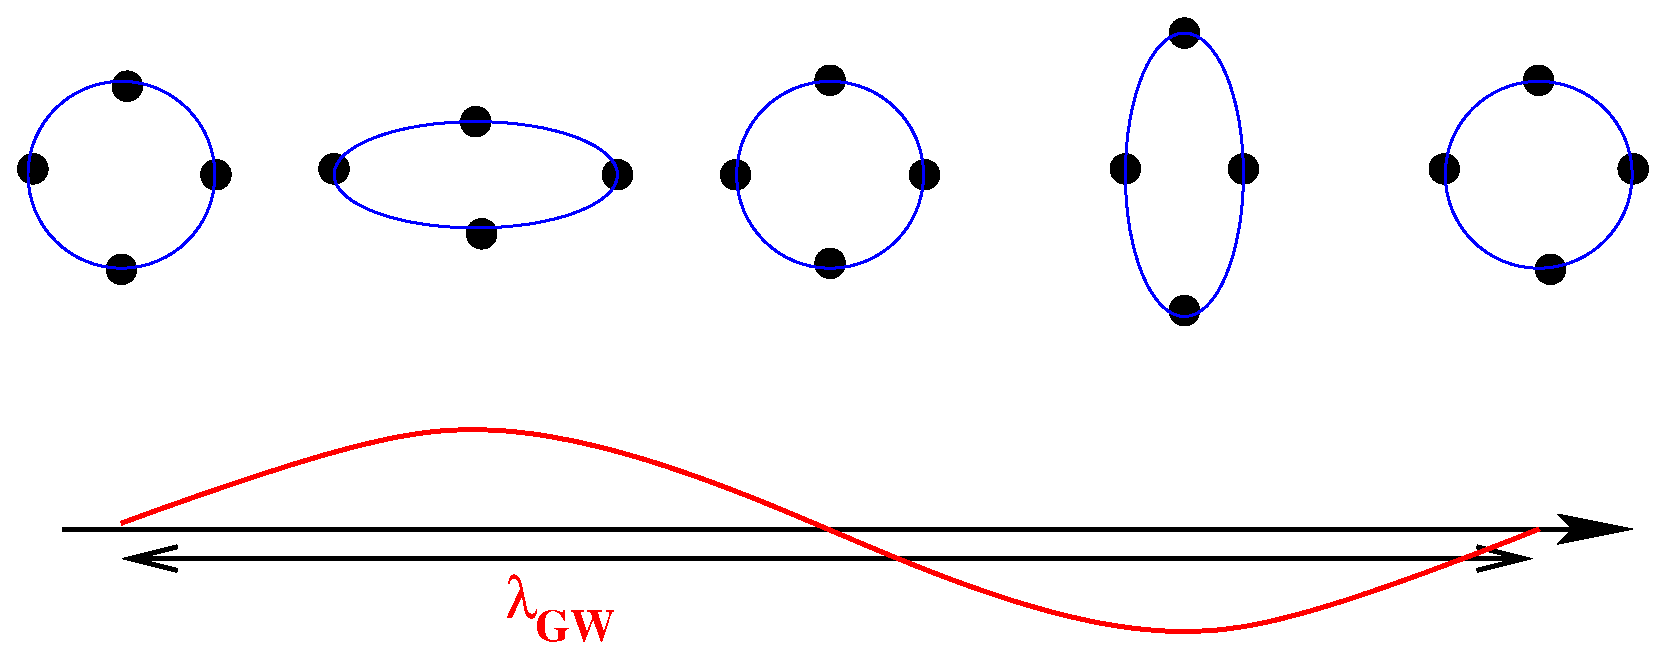
\includegraphics[width=.95\linewidth]{intro/GW1}
\end{subfigure}
\begin{subfigure}{.80\textwidth}
  \centering
  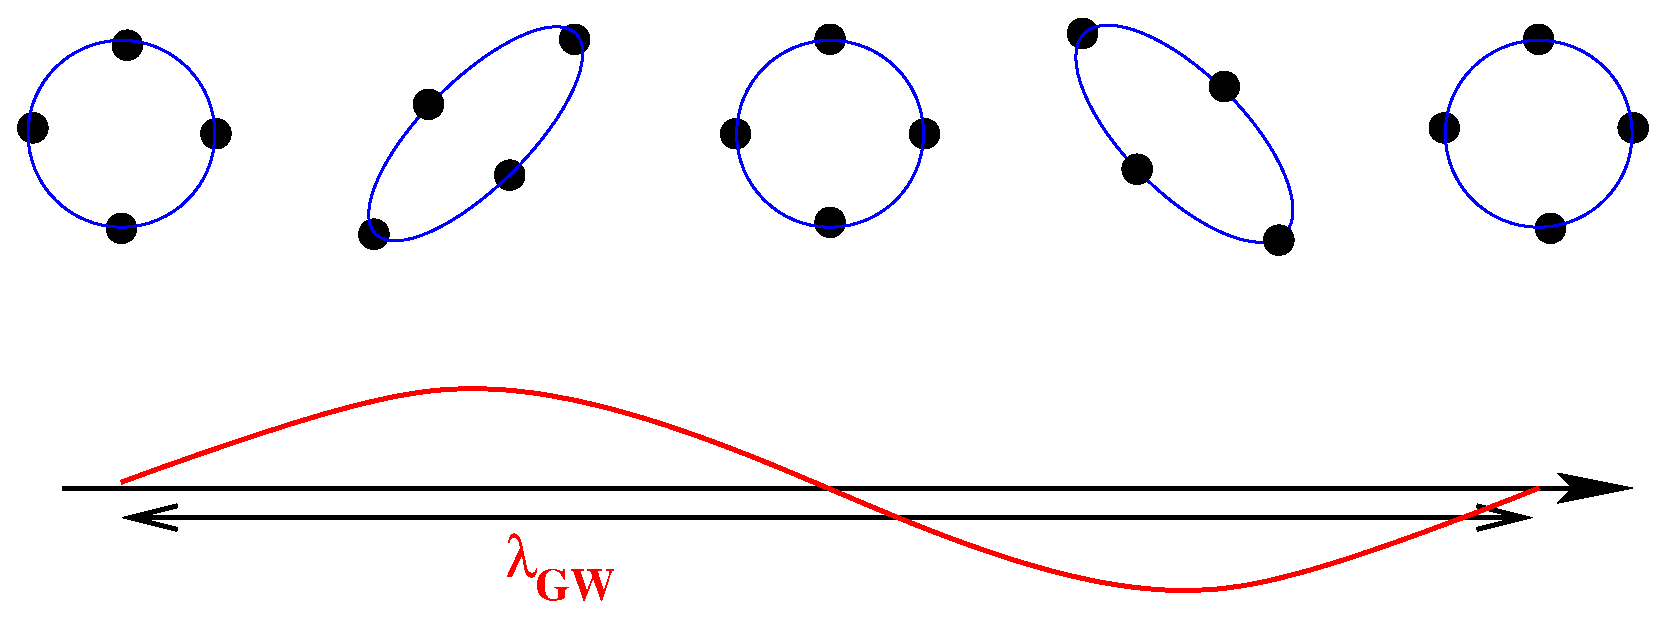
\includegraphics[width=.95\linewidth]{intro/GW2}
\end{subfigure}
\caption[Effect of gravitational waves on a ring of particles.]{From~\cite{Buonanno:2007yg}. The top panel shows the effect of a $+$ polarized gravitational wave passing through a ring of particles, in the direction perpendicular to the plane of the ring. The bottom panel shows the effect of a $\times$ polarized gravitational wave.}
\label{fig:GWRing}
\end{figure}

When a matter source is present, the wave equation becomes
\begin{equation}
\nabla_{\rho}\nabla^{\rho}h_{\munu}=-16\pi T_{\munu}.
\end{equation}
The solution to this equation can be written with the help of a Green's function,
\begin{equation}
h_{\munu}(t,x^{i})=4\int{d^3y\frac{1}{|x-y|}T_{\munu}(t_r,y^i)},
\end{equation}
where $t_r$ is the ``retarded'' time, $t_r=t-|x-y|$. This integral can be evaluated in terms of the quadruople tensor $I^{ij}$ defined by
\begin{equation}
I^{ij}(t)=\int{d^3x x^ix^jT^{00}(t,x^i)},
\end{equation}
and the reduced quadrupole moment
\begin{equation}
J_{ij}=I_{ij}-\frac{1}{3}\eta_{ij}I,
\end{equation}
where $I=I^{\mu}_{\mu}$.
The result is
\begin{equation}
h_{ij}(t,x^i)=\frac{2}{r}\ddot{J}_{ij}^{\ttt}(t_r)
\end{equation}
In other words, linear gravitational waves are sourced by an oscillating quadrupole. To study the energy content of these gravitational waves, note that the effective stress-energy tensor of this spacetime is
\begin{equation}
T_{\munu}=\frac{1}{32\pi}\left<\partial_{\mu}h_{ij}\partial_{\nu}h^{ij}\right>.
\end{equation}
This can be integrated to find the energy output per unit time in gravitational waves,
\begin{eqnarray}
\label{eq:LGW}
L_{GW}&=&\frac{r^2}{16\pi}\oint{\left<\dot{h}_{\times}^2+\dot{h}_{+}^2\right>d\Omega}\\
&=&\frac{1}{5}\left<\dddot{J}_{ij}^{\ttt}\dddot{J}^{\ttt ij}\right>.
\end{eqnarray}
Let us now consider a circular binary with total mass $M$, reduced mass $\mu$, separation $R$ and orbital frequency $\omega$. Direct computation of the quadrupole tensor gives the simple result
\begin{equation}
L_{GW}=\frac{32}{5}\mu^2M^3R^{-5}.
\end{equation}
Using this, along with the Newtonian estimates $\omega=M^{1/2}R^{-3/2}$, $E=-\frac{\mu M}{2R}$, $dE/dt=-L_{\rm GW}$, allows us the compute the characteristic inspiral scales. The binary shrinks at a rate
\begin{equation}
\frac{dR}{dt}=\frac{dE/dt}{dE/dr}=\frac{-64}{5}M^2\mu R^{-3}.
\end{equation}
Integrating this expression gives the time to coallescence where $R=0$ as
\begin{equation}
\tau_{c}=\frac{5}{256}M^{-2}\mu^{-1}R^{4}.
\end{equation}
As the binary separation decreases, the orbital frequency increases. By integrating
\begin{equation}
\frac{df_{\rm{GW}}}{dt}=\frac{1}{\pi}\frac{d\omega}{dt}=\frac{-3M^{1/2}}{2}R^{-5/2}\frac{dR}{dt},
\end{equation}
the frequency evolution is given by
\begin{equation}
f_{\rm{GW}}(t) = \frac{\omega}{\pi}=\frac{1}{8\pi}\left(\frac{5}{\mu M^{2/3}(\tau_{c}-t)}\right)^{3/8}.
\end{equation}
The number of gravitational waves cycles, $N=\int{f_{\rm{GW}}dt}$, in a given frequency band $df_{\rm{GW}}$ is given by
\begin{equation}
\frac{dN}{d\log{f_{\rm{GW}}}}=\frac{5}{96\pi}\frac{1}{\left(\pi\mathcal{M}f_{\rm{GW}}\right)^{5/3}},
\end{equation}
where the quantity $\mathcal{M}=\mu^{3/5}M^{2/5}$ is called the ``chirp mass''. The explicit radiation pattern is given by
\begin{eqnarray}
h_{+} &=& \frac{4}{r}\mathcal{M}^{5/3}(2\omega)^{2/3}\cos(2\omega t+\phi)\left(\frac{1+\cos^2\theta}{2}\right), \\
h_{\times} &=& \frac{4}{r}\mathcal{M}^{5/3}(2\omega)^{2/3}\sin(2\omega t +\phi)\cos\theta,
\end{eqnarray}
where $r$ is the distance to the source, $\theta$ is the angle between the observer and the axis normal to the orbital plane of the binary, and $\phi$ is the arbitrary phase of the binary. Detectors are sensitive to the strain $h$, rather than the energy flux, and therefore a factor of $x$ improvement in sensitivity results in a factor of $x^3$ higher event rate (assuming a uniformly placed distribution of sources).

These estimates were all made for a circular binary. If the binary has some eccentricity, $e$, then equation~\ref{eq:LGW} is modified to
\begin{equation}
L_{GW}=\frac{32}{5}\mu^2M^3R^{-5}\left(1+\frac{73}{24}e^2+\frac{37}{96}e^4\right)\left(1-e^2\right)^{-7/2}
\end{equation}
However, eccentriccity is radiated away as the inspiral proceeds. The classic reference of Peters(1964) found that
\begin{equation}
\left<\frac{de}{dt}\right>=-\frac{304}{15}e\frac{\mu M^2}{R^4\left(1-e^2\right)^{5/2}}\left(1+\frac{121}{304}e^2\right).
\end{equation}
Thus even a highly eccentric binary will radiate away its eccentricity and circularize before merger, provided the compact objects started far enough away from each other. Most numerical relativity simulations consider only circularized binaries and use techniques to attempt to get rid of any residual eccentricity.

The equations above in this section are valid only for a slowly-moving, weak-field system. As the system gets closer and closer to merger, these equations become increasingly inacurate. Post-Newtonian theory, by expanding to higher order, allows us to consider binaries with higher orbital frequencies. It is typically written as an expansion in the dimensionless parameter 
\begin{equation}
x=\left(\frac{GM\omega}{c^3}\right)^{(2/3)}.
\end{equation}
The evolution of the orbital phase, for example, can be written as
\begin{equation}
\phi=\frac{-x^{-5/2}}{32\nu}\left(1+a_1x + a_2x^{3/2} + a_3x^2 + a_4x^{5/2} + a_5x^3 + a_6x^{7/2}+\mathcal{O}(1/c^8)\right)
\end{equation}
where $\nu$ is the symmetric mass ratio, $\nu=\frac{m_1m_2}{(m_1+m_2)^2}$, and each of the $a_i$ are functions only of $\nu$ and $\log{x}$. This expression is said to be known to 3.5 Post-Newontian order. Additional contrbutions come in at other PN orders, such as spin-orbit coupling at 1.5 PN order, spin-spin coupling at 2 PN order and tidal effects at 5 PN order. See~\cite{Blanchet2006} and references therein for an overview of PN results and methodology.


\section{The initial value problem in Numerical Relativity}
\label{sec:IVP}
From the point of view of numerical relativity, it is natural to use a 3+1 decomposition of space-time. In this section, we will review this process. Given a globally hyperbolic spacetime $(M,g_{\munu})$. We foliate $M$ by a set of $t={\rm const}$ hypersurfaces $\Sigma_t$. This is illustrated in Fig.~\ref{fig_Slice}.
\begin{center}
\begin{figure}[!ht]
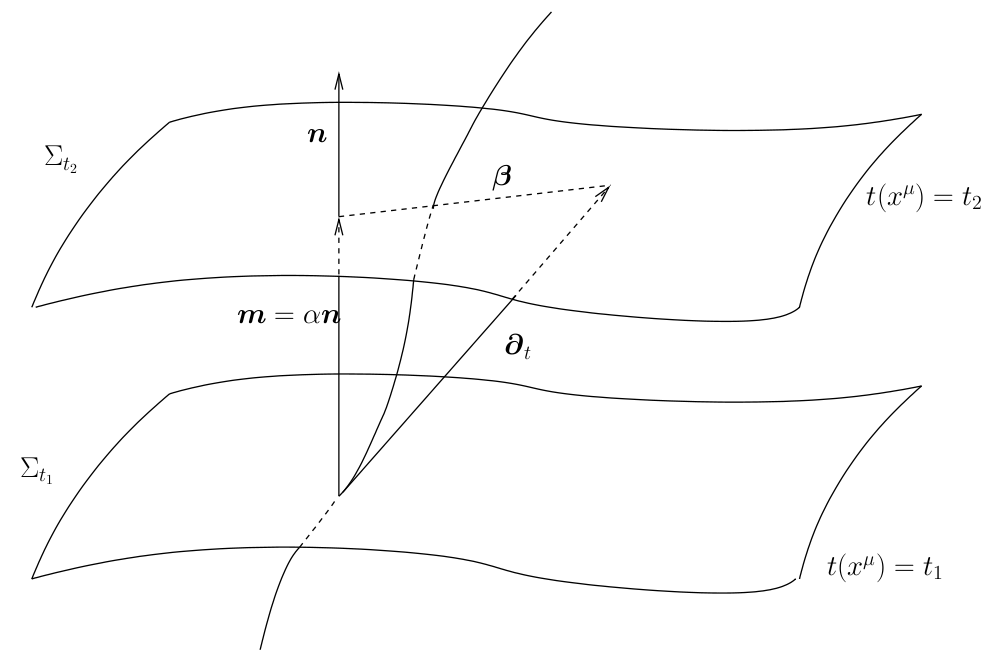
\includegraphics[scale=0.45]{intro/Slice.png}
\caption[Illustration of the 3+1 decomposition.]{From~\cite{Cardoso2014}. An illustration of the foliation of spacetime by space-like hypersurfaces $\Sigma_t$, as well as illustrating the lapse, $\alpha$, the shift, $\beta^i$, and the normal $n^{\mu}$.}
\label{fig_Slice}
\end{figure}
\end{center}

 Each surface has a forward pointing unit normal
\begin{equation}
n^{\mu}=-g^{\munu}\nabla_{\nu}t\left(g^{\munu}\nabla_{\mu}t\nabla_{\nu}t\right)^{-1/2},
\end{equation}
induced metric
\begin{equation}
\gamma_{\munu}=g_{\munu}+n_{\mu}n_{\nu},
\end{equation}
and compatible derivative operator $D$.
The induced metric measure curvature inside each hypersurface, while the extrinsic curvature $K_{\munu}$ measures how the hypersurface is curved insde the space-time manifold $M$. It is defined by 
\begin{equation}
K_{\munu}=-\frac{1}{2}\mathcal{L}_{n}g_{\munu},
\end{equation}
where $\mathcal{L}_n$ is the usual Lie derivative, along the direction of the vector field $n^{\mu}$.
The space-time metric is written as
\begin{equation}
ds^2=-\alpha^2dt^2 + \gamma_{ij}\left(dx^i+\beta^idt\right)\left(dx^j+\beta^jdt\right).
\end{equation}
Here $\alpha$ is known as the lapse function - it measures the proper time between neighbouring hypersurfaces. $\beta^i$ is known as the shift - it measures the proper distance within a spatial hypersurface. The lapse and shift are both arbitrary - their choice amounts to a choice of coordinates.

Similar to how Maxwell's equations can be written as a set of constraint equations that do not contain any time derivatives,
\begin{eqnarray}
D_iE^i -4\pi\rho &=& 0, \\
D_iB^i &=& 0,
\end{eqnarray}
and evolution equations,
\begin{eqnarray}
\partial_tE_i&=&\epsilon_{ijk}D^jB^k - 4\pi j_i\\
\partial_tB_i&=&-\epsilon_{ijk}D^jE^k,
\end{eqnarray}
(where $E^i$ is the electric field, $B^i$ is the magnetic field, $\rho$ is the charge density, $j^i$ is the current density, and $\epsilon_{ijk}$ is the Levi-Civitia symbol, and the equations are written in Gaussian units), the same is true of Einstein's equations. The famous Hamiltonian and momentum constraints are
\begin{equation}
R+K^2-K_{ij}K^{ij}=16\pi\rho,
\end{equation}
and,
\begin{equation}
D_{j}K^{j}_{i}-D_iK=8\pi S_i
\end{equation}
where $\rho$ is the energy density measured by a normal observer, $\rho=n_in_jT^{ij}$, and $S_i$ is the momentum density measured by a normal observer $S_i=-\gamma^{j}_in^kT_{jk}$. These are elliptic equations for the geometric quantities defined on the $\Sigma_t$. The general task of constructing initial data is to find ($\Sigma, g_{\munu}, K_{\munu}$) that satisfy the constraint equations and represent well the physical situation at hand (e.g., the inspiral of a compact object binary). The evolution equations are
\begin{equation}
\partial_t\gamma_{ij}=-2\alpha K_{ij} + D_{i}\beta_j + D_j\beta_i
\end{equation}
and
\begin{equation}
\partial_tK_{ij}=-D_iD_j\alpha + \alpha\left(R_{ij}-2K_{ik}K^k_j+KK_{ij}\right)\\
-8\pi\alpha(S_{ij}-\frac{1}{2}\gamma_{ij}(S-\rho))+\beta^kD_kK_{ij}+K_{ik}D_j\beta^k+K_{kj}D_i\beta^k
\end{equation},
where $S_{ab}$ is the spatial stress, $S_{ab}=\gamma^c_a\gamma^d_bT_{cd}$, and $S$ is its trace. Once constraint satisfying initial data has been constructed, the evolution equations determine the geometric quantities at all future times. Analytically, the evolution equations preserve the constraints, although numerically this may not always be the case. 

There are many sets of data $(g_{\munu},K_{\munu})$ that will satisfy the constraint equations. The task remains, then, to choose this free data appropriately. To do so, one typically begins with a conformal decomposition of the metric,
\begin{equation}
\gamma_{ij}=\Psi^4\tilde{\gamma}_{ij}.
\end{equation}
Here, $\Psi$ is called the conformal factor, and $\tilde{\gamma}_{ij}$ is called the conformal metric. Next we break up the extrinsic curvature into its trace and trace-free parts,
\begin{equation}
K_{ij}=A_{ij}+\frac{1}{3}\gamma_{ij}K.
\end{equation}
The Hamiltonian and Momentum constraints become
\begin{equation}
\tilde{D}^2\Psi-\frac{1}{8}\Psi\tilde{R}-\frac{1}{12}\Psi^5K^2+\frac{1}{8}\Psi^{-5}\tilde{A}_{ij}\tilde{A}^{ij}=-2\pi\Psi^{-5}{\rho}.
\end{equation}
\begin{equation}
{D}_j{A}^{ij}-\frac{2}{3}{D}^iK=8\pi j^i,
\end{equation}

$\tilde{A}^{ij}=\Psi^{-10}A^{ij}$. We now proceed according to the extended conformal thin sandwich formalism. We define 
\begin{equation}
\tilde{u}_{ij}=\partial_t\tilde{\gamma}_{ij},
\end{equation}
and we introduce the scalings
\begin{eqnarray}
\tilde{j}^i &=& \Psi^{10}j^i, \\
\tilde{\rho} &=& \Psi^{8}\rho \\
\tilde{A}^{ij} &=& \Psi^{10} A^{ij}. 
\end{eqnarray}
The Hamiltonian and Momentum constraints constraints can now be viewed as equations for the shift and conformal factor
\begin{equation}
\tilde{D}^2\Psi-\frac{1}{8}\Psi\tilde{R}-\frac{1}{12}\Psi^5K^2+\frac{1}{8}\Psi^{-7}\tilde{A}_{ij}\tilde{A}^{ij}=-2\pi\Psi^{-3}\tilde{\rho},
\end{equation}
\begin{equation}
\tilde{D}_j\left(\frac{1}{2\tilde{\alpha}}\left(\mathbb{L}\beta\right)^{ij}-\tilde{D}_j\left(\frac{1}{2\tilde{\alpha}}\tilde{u}^{ij}\right)\right)-\frac{2}{3}\Psi^6\tilde{D}^iK=8\pi\tilde{j}^i,
\end{equation}
where
\begin{equation}
\tilde{\alpha}=\Psi^6\alpha
\end{equation}
is the conformal lapse and 
\begin{equation}
\left(\tilde{\mathbb{L}}\beta\right)^{ij}=\Psi^4\left(D^i\beta^j+D^j\beta^i-\frac{2}{3}\gamma^{ij}D_k\beta^k\right)
\end{equation}
is the conformal longitudinal operator. The lapse is given by the evolution equation of $K$,
\begin{eqnarray}
&&\tilde{D}^2\left(\tilde{\alpha}\Psi^7\right) -
\left(\tilde{\alpha}\Psi^7\right)\bigg[\frac{1}{8}\tilde{R}+\frac{5}{12}\Psi^4K^2+\frac{7}{8}\Psi^{-8}\tilde{A}_{ij}\tilde{A}^{ij}\nonumber \\
\label{eq:XCTS-Lapse}
&&+2\pi\Psi^{-2}\big(\tilde{E}+2\tilde{S}\big)\bigg]=-\Psi^5\left(\partial_{t}K
- \beta^{k}D_kK\right).
\end{eqnarray}
The free data are $\tilde{\gamma}_{ij},\tilde{u}_{ij},K,\partial_tK$. In a coordinate system corotating with the binary, it is natural to choose $\tilde{u}_{ij}=0, \partial_tK=0$. Common choices are conformal flatness, $\tilde{\gamma}_{ij}=\delta_{ij}$ and maximal slicing $K=0$. With appropriate boundary conditions, the system of equations can now be solved.

\section{Binary Neutron Star Systems}
\label{sec:BNS}

%\subsection{Binary Neutron Star Formation}
To begin our discussion of the properties of binary neutron star binaries, we should first briefly review how these system forms. We follow the discussion outlined in \cite{Postnov:2014tza}. The standard formation scenario is illustrated in figure~\ref{fig_BinaryEvolution}, and goes as follows:

\begin{itemize}

\item We begin with two high mass OB main-sequence stars undergoing standard binary evolution. Eventually the more massive (primary) star burns its central hydrogen, and a helium core is left over. 

\item The primary star then rapidly expands, overflows its Roche lobe, and begins a period of mass transfer onto the secondary star. This period lasts until most of the primary's Hydrogen envelope has been transferred, leaving behind a naked helium core.

\item The primary star eventually collapses as a core-collapse supernova, leaving behind a neutron star. It is likely that the explosion disrupts the binary, but let us assume that it survives. We then have a massive main sequence star in orbit with a neutron star.

\item Eventually the secondary star evolves off the main sequence, expands, and overflows its Roche lobe. It will then begin accreting mass onto the primary. This accretion spins up the neutron star, thus ``recycling" it. It also leads to strong x-ray emission.

\item The secondary further expands and a common envelope stage ensues. Eventually the secondary explodes as a supernova, and becomes a neutron star.

\item If the system is not disrupted, it can then become a binary that will eventually merge due to the continuous emission of gravitational waves.

\end{itemize}

\begin{figure}[!ht]
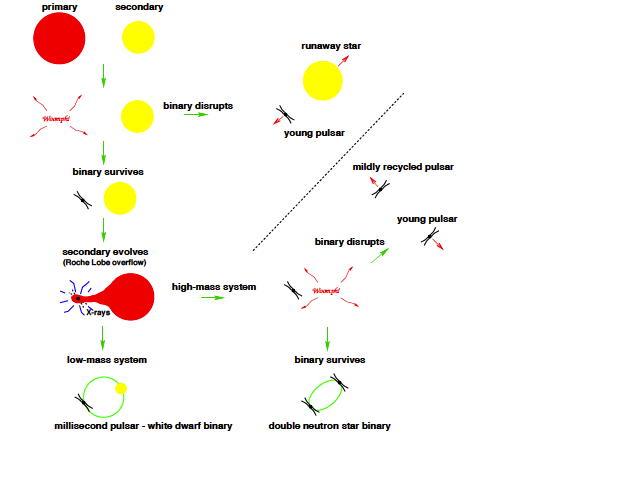
\includegraphics[scale=0.95]{intro/BinaryEvolution.png}
\caption[Evolutionary scenarios of a typical high-mass binary.]{From \cite{Lorimer2008}. The possible evolutionary scenarios of a typical high mass binary are shown.}
\label{fig_BinaryEvolution}
\end{figure}

As discussed earlier, such systems are expected to be quasi-circular once they enter the LIGO band. There are, however, other ways of forming systems that are highly eccentric while in the LIGO band. For example, the dynamical capture in a close two-body encounter in a dense cluster environment, or a binary in a hierarchichal triple system whose eccentricity is enhanced by the Kozai mechanism. Nonetheless, quasi-circular binaries are expected to constitute the large majority of gravitational wave sources.

%NS-NS binaries, unlike BH-BH and BH-NS binaries, have been observed and studied within our galaxy, and therefore the expectations of ground-based gravitational wave detectors for NS-NS binaries are more tightly constrained. The known binary neutron star population is summarized in table~\ref{tab:KnownBNS}
%We report the spin periods, orbital periods, eccentricities, characteristic ages ($\tau_c=P/\dot{P}$), time until coalescence through gravitational wave emission, $\tau_g$. For systems that merge in a Hubble time, we also list the final spin of the star, $P_f$. Assuming magnetic dipole spin-down from a constant magnetic field, this is given by 
%\begin{equation}
%P_f = P\sqrt{1+\frac{\tau_g}{\tau_c}}.
%\end{equation}
% \begin{table}
% \centering
%\label{tab:KnownBNS}
% \caption{The properties of known double neutron star systems}
% \begin{tabular}{c || c | c | c | c | c | c}
% \hline
% System & $P(ms)$ & $P_{\textnormal{orb}}(d)$ & $e$ & $\log_{10}{\tau_c(yr)}$ & $\log_{10}{\tau_g(yr)}$ & $P_f(ms)$ \\
% \hline \hline
% J0737-3039 & 22.7 & 0.102 & 0.088 & 8.3 & 7.9 & 26.8 \\
% J0737-3039 &  2770 & 0.102 & 0.088 & 7.7 & 7.9 &   4453 \\
% J1518+4904 & 40.9 & 8.6 & 0.25 & 10.3 & 12.4 & --- \\
% B1534+12 & 37.9 & 0.32 & 0.27 & 8.4 & 9.4 & 126 \\
% J1756-2251 & 28.5 & 0.32 & 0.18 & 8.6 & 10.2 & --- \\
% J1811-1736 & 104.2 & 18.8 & 0.83 & 9.0 & 13.0 & --- \\
% B1820-11 & 279.8 & 357.8 & 0.79 & 6.5 & 15.8 & --- \\
% J1829+2456 & 41.0 & 1.18 & 0.14 & 10.1 & 10.8 & --- \\
% J1906+0746 & 144.1 & 0.17 & 0.085 & 5.1 & 8.5 & 7224 \\
% B1913+16 & 59.0 & 0.3 & 0.62 & 8.0 & 8.5 & 120 \\
% B2127+11C & 30.5 & 0.3 & 0.67 & 8.0 & 8.3 & 52.6 \\ 
% \end{tabular}
 %\end{table}

The end state of a binary neutron star merger depends strongly on the properties of the stars. For systems with a combined mass less than the maximum mass allowed by the EOS, the final result would be a more massive neutron star. Otherwise, the final result will be a single Kerr black hole. Simulations have shown that these black holes will have a spin on the order of $\chi \simeq 0.6-0.8$. The intermediate state is known as a hypermassive neutron star (HMNS). This is a NS whose mass is above the maximum mass allowed by the EOS, temporarily supported by differential rotation and thermal pressure. Over time, angular momentum is efficiently transported out of the system, and it collapses into a black hole. We can further subdivide these systems based on the timescale for callapse - prompt collapse or delayed collapse. In the prompt case, the pressure support is too low, and the system collapses on a $\sim$ freefall timescale. This is expected in systems with a large total mass ($\gtrsim 2.8M_{\odot}$), although the details depend, of course, on the EOS. In the delayed collapse case, the collapse timescale depends on many factors. Angular momentum distribution by magnetic winding is an important factor - it operates on the Alfven timescale $\tau \sim R\sqrt{\rho}/B \simeq 10-100{\rm ms}$. Transport driven by magneto-rotational instability is also important. It is of the order $\tau \sim 100{\rm ms}$ for $B \simeq 10^{15}G$. Cooling by neutrino or electromagnetic emission is also important, as it decreases thermal pressure, although it operates on a longer timescale, $\sim$ seconds. An accretion disk around the eventual BH, lying beyond the ISCO, will form, with a mass of $\simeq 0.01-0.3 M_{\odot}$. The amount of material in the disk depends on the time to BH formation, as there is more time to distribute angular momentum ot the disk. HMNS systems emit gravitational waves at peak frequencies of approximately $2-4 {\rm kHz}$ (see, e.g.,~\cite{Hotokezaka:2011dh}), unfortunately outside of the optimal frequency range of ground-based detectors. 

The mass ratio of the system is another important factor. Figure ~\ref{fig:Contours} shows the post-merger remnant of an equal-mass system, and of a system with mass ratio $q\sim 1.38$~\citep{Rezzolla:2010fd}. The equal mass system shows a ``dumbell''-like structure, composed of two cores which, over time, turn into an ellipsoidal HMNS. The non-equal-mass case shows two asymmetric cores, which act like the smaller one orbiting the larger one. The stronger tidal forces in this case cause the outher layers of the smaller star to be stripped off and form an envelope around the HMNS. Higher disk mass correlates with higher deviations from $q=1$, as well as with higher NS compactness.

\begin{figure}[!t]
\centering
\begin{subfigure}{.80\textwidth}
  \centering
  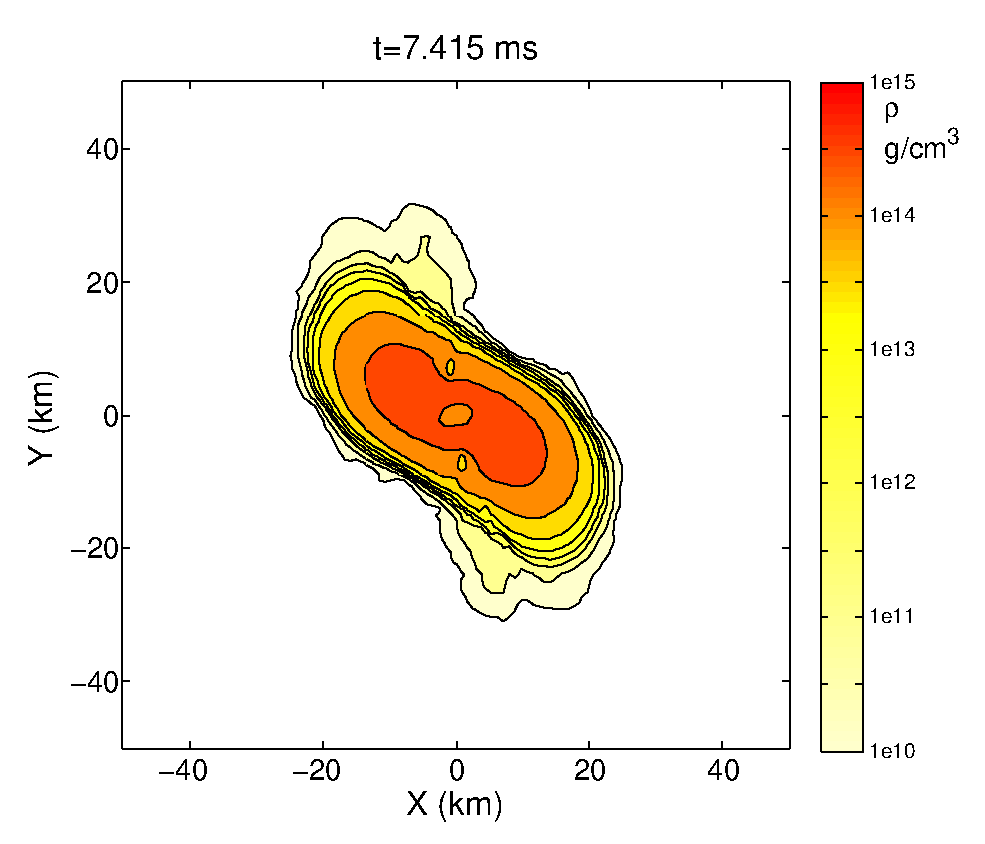
\includegraphics[width=.95\linewidth]{intro/Contours1}
\end{subfigure}
\begin{subfigure}{.80\textwidth}
  \centering
  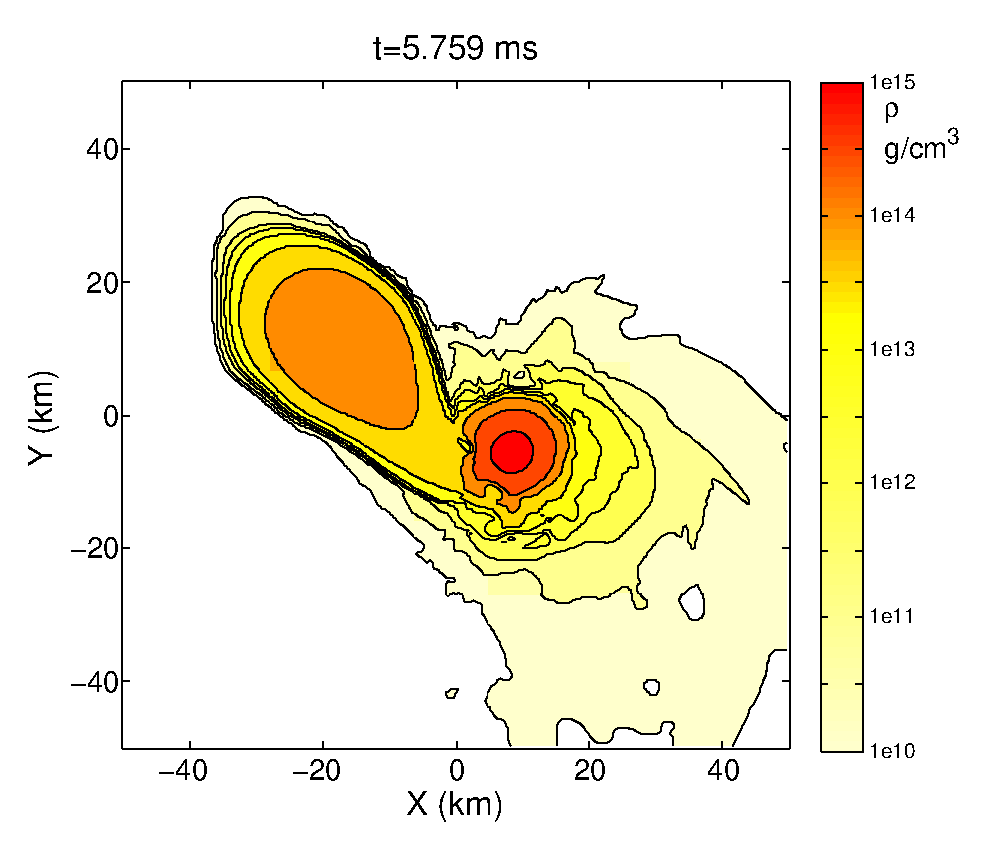
\includegraphics[width=.95\linewidth]{intro/Contours2}
\end{subfigure}
\caption[Comparison of an equal mass BNS system and a non-equal mass BNS system.]{From ~\cite{Rezzolla:2010fd}. The top panel shows the iso-density contours of the HMNS from an equal mass system with baryon masses $M_1=M_2=1.643M_{\odot}$. The bottom panel shows the iso-density contours of the HMNS from a system with baryon masses $M_1=1.304M_{\odot}$ and $M_2=1.805M_{\odot}$.}
\label{fig:Contours}
\end{figure}

The merger of two neutron stars is the site of the emission of a tremendous amount of electromagnetic energy. Their mergers are thought to be one of the most promising candidates to be the progenitors of short gamma ray bursts (SGRBs), although there is not yet definitive evidence of it. The engine of a rotating black hole, surrounded by a hot accretion torus and a collimiated magnetic field contains the necessary ingreidients thought to be needed for a SGRB. Apart from this, another promising candidate for electromagnetic signature is the ``kilonova'' - emission powered by the radioactive decay of r-process elements formed in the merger, lasting on the time-scale of $\sim$ weeks. Multi-messenger astronomy (see \cite{Fan:2015bia} for a review) seeks to combine information from gravitational waves, these electromagnetic events, and possible neutrino observations, to further elucidate the astrophysics of these mergers.

One of the most exciting prospects of the Advanced LIGO era is using gravitational wave observations to constrain the NS EOS. The EOS of dense nuclear matter is an open question of tremendous interest to nuclear physicists and astrophysicists alike. Tidal effects are parameterized by the tidal deformability paramter $\lambda$, which relates the induced quadrupole field of one star, $Q_{ij}$, to the tidal field in which it is immersed, $\mathcal{E}_{ij}$:
\begin{equation}
Q_{ij}=-\lambda(m;{\rm EOS})\mathcal{E}_{ij}.
\end{equation}
Or, likewise, by the second tidal Love number,
\begin{equation}
k_2=\frac{3}{2}\frac{\lambda}{R^5}.
\end{equation}
These enter the PN equations for binary phase at the very high 5PN order, but because of the large pre-factors, they are still very important in the late-stage inspiral dynamics. Much work has been done to estimate how well Advanced LIGO can measure these paramters (see ~\cite{Read2009b,Hinderer2010,damour:12,Lackey2011}). \cite{DelPozzo:13} (further extended in~\cite{Agathos:2015a}) used a Bayesian framework to show that $\lambda$ could be constrained at the 10\% level after a few tens of detections. There is also the question of more exotic NS matter. \cite{Chatziioannou:2015uea} studied various possibilities and found, for example, that a detection with an SNR of $\sim 20$ could provide good evidence of the existence or non-existence of strange quark stars.

Numerical simulations of the mergers of binary neutron stars have been possible for at least fifteen years~\citep{Shibata00b}. Since then, simulations have rapidly progressed, by adding more resolution~\citep{Hotokezaka2013}, more orbits~\citep{Haas:2016}, radiative losses~\citep{Kiuchi:2012mk,Neilsen:2014hha,Palenzuela2015,Sekiguchi:2015}, studying different equations of state~\citep{Hotokezaka:2011dh,Kiuchi:2012mk,Neilsen:2014hha}, magnetic fields~\citep{Liu:2008xy,Giacomazzo:2010bx,Rezzolla:2011da,Anderson:2008zp,Neilsen:2014hha,Kiuchi2015,PalenzuelaEtAl:2013,Palenzuela:2013kra,2015arXiv150202021D}, unequal mass ratios~\citep{Rezzolla:2010fd,Kiuchi:2010ze,Shibata:2003ga,Dietrich:2015iva},ejecta~\citep{Wanajo2014,Sekiguchi:2015,RadiceLeak:2016} eccentric binaries~\citep{Gold:2011df}, and spinning binaries~\cite{Bernuzzi:2013rza,Kastaun:2013mv,Dietrich:2015pxa,Tacik:2015tja}. Note that this is by no means an exhaustive list of ongoing research -- see~\cite{Baiotti:2016qnr} for an up-to-date review. With the great increase in simulation technology, and the coincident start of the Advanced LIGO era, it is truly an exciting time for this field.

%\section{Astrophysical Motivation}

%\subsection{How Important is Spin?}
%The obvious first question to ask is, ``what spin is necessary to be relevant in a binary neutron star simulation?" After answering that, we will then ask, ``are there realistic astrophysical scenarios that would produce such spins?''

%Our first approach is just a simple comparison of time scales. The two relevant time scales in the problem are the orbital period, $P_{\textnormal{orb}}$, and the spin period, $P$. If $P_{\textnormal{orb}}\ll P$, then the spin can be safely neglected, but if this condition is false, then the spin may be important. Kepler's third law gives
%\begin{equation}
%P_{\textnormal{orb}}^2=\frac{4\pi^2a^3}{M}
%\end{equation}
%Suppose the neutron stars are close to merger, say, $a=45km$. If we take $M=2.8M_{\odot}$, then the orbital period is $P_{\textnormal{orb}}\approx 3ms$. If the $\ll$ criterion is taken to be an order of magnitude, we can then conclude that neutron stars with a spin period on the order of a few dozen milliseconds might be non-negligible.

%Next, we can investigate how much the neutron star spin can affect the accumulated orbital phase of the system. Consider an equal mass system, where one of the neutron stars has dimensionless spin $\chi=\frac{J}{M^2}$ aligned with the orbital momentum. Boyle et. al. (2007)\cite{BoyleEtAl2007} gives the accumulated phase difference, due to spin-orbit coupling, computed at 2.5 Post-Newtonian order, as a function of $x=a/M$ as
%\begin{equation}
%\Phi\approx -\chi\left(\frac{1.22}{x}-8.5\log{x}\right)
%\end{equation}
%If we want to compute the phase error accumulated in LIGO's most sensitive region for binary neutron stars, say 40Hz-400Hz \cite{AndersonCreighton2008}, this corresponds to finding the difference between $x=0.0144$ and $x=0.067$. The result is
%\begin{equation}
%\delta\Phi \approx -80\chi
%\end{equation}
%The error in the waveform phase is just twice the orbital phase,
%\begin{equation}
%\delta\phi \approx -160\chi
%\end{equation}
%If we take the neutron star's angular momentum to be $J=\frac{2}{5}MR^2\Omega$, then its dimensionless spin is
%\begin{equation}
%\chi = \left(\frac{R}{15km}\right)^2\left(\frac{1.4M_{\odot}}{m}\right)\left(\frac{1ms}{P}\right)
%\end{equation}
%and the phase error is then
%\begin{equation}
%\delta\phi = 10rad \left(\frac{R}{15km}\right)^2\left(\frac{1.4M_{\odot}}{m}\right)\left(\frac{16ms}{P}\right)
%\end{equation}

%Finally, let us make a crude estimate on the effect of the disk mass after the merger due to neutral star spin. This can crudely be done by assuming all of the spin angular momentum of the neutron star goes into the disk, i.e., we set
%\begin{equation}
%J_{NS} = J_{D}
%\end{equation}
%\begin{equation}
%\frac{4\pi}{5}\frac{M_{NS}R_{NS}^2}{P} = \frac{1}{2}M_DR_D^2\Omega_{D}
%\end{equation}
%Let's assume that the remnant mass is $2M_{NS}$ and that $R_D=fM_{\textnormal{Remnant}}$ for some real number $f$. We then obtain that the disk mass is
%\begin{equation}
%M_D = \frac{4\pi}{5\sqrt{f}}\frac{R_{NS}^2}{P}
%\end{equation}
%If we take $f=6$ as for non-rotating black holes, we obtain
%\begin{equation}
%M_D = 0.005M_{\odot}\left(\frac{R}{15km}\right)^2\left(\frac{P}{10ms}\right)^{-1}
%\end{equation}
%This mass could easily be enhanced by adding a small deviation away from equal mass ratio, and give the mass necessary to be the engine of short GRBs.

%Although these are not completely precise arguments, the take away message here should be that neutron stars with spins on the order of a couple tens of milliseconds should not be neglected in simulations.

%\subsection{Binary Neutron Star Formation}
%To begin our discussion of the properties of binary neutron star binaries, we should first briefly review how these system forms. We follow the discussion outlined in \cite{PostnovYungelson2006}. The standard formation scenario is illustrated in figure 1courtesy of \cite{Lorimer2008}, and goes as follows:

%\begin{itemize}

%\item We begin with two high mass OB main-sequence stars undergoing standard binary evolution. Eventually the more massive (primary) star burns its central hydrogen, and a helium core is left over. 

%\item The primary star then rapidly expands, overflows its Roche lobe, and begins a period of mass transfer onto the secondary star. This period lasts until most of the primary's Hydrogen envelope has been transferred, leaving behind a naked helium core.

%\item The primary star eventually collapses as a core-collapse supernova, leaving behind a neutron star. It is likely that the explosion disrupts the binary, but let us assume that it survives. We then have a massive main sequence star in orbit with a neutron star.

%\item Eventually the secondary star evolves off the main sequence, expands, and overflows its Roche lobe. It will then begin accreting mass onto the primary. This accretion spins up the neutron star, thus ``recycling" it. It also leads to strong x-ray emission.

%\item The secondary further expands and a common envelope stage ensues. Eventually the secondary explodes as a supernova, and becomes a neutron star.

%\item If the system is not disrupted, it can then become a binary that will eventually merge due to the continuous emission of gravitational waves.

%\end{itemize}

%\begin{figure}[!ht]
%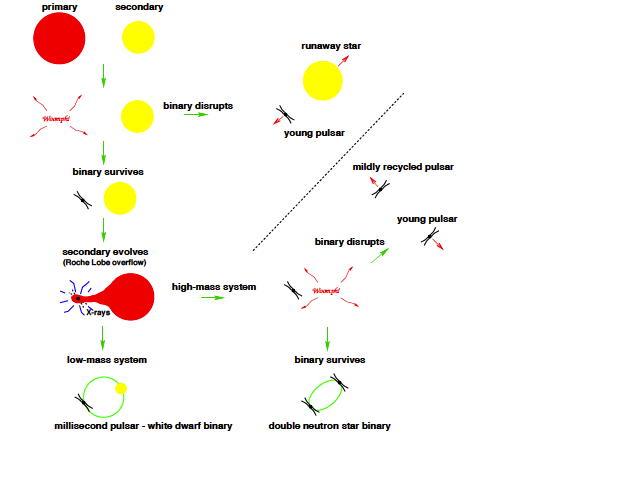
\includegraphics[scale=0.75]{intro/BinaryEvolution.png}
%\label{fig_BinaryEvolution}
%\caption{Courtesy of \cite{Lorimer2008}. The possible evolutionary scenarios of a typical high mass binary are shown}
%\end{figure}

%\subsection{Why Corotation is Unphysical}
%In principle, neutron stars in compact binaries could perhaps be spun up to coronation by tidal torques. The argument that they are not is outlined in \cite{BildstenCutler1992}. Consider a binary consisting of a neutron of mass $m$ and radius $R$, with a companion (either a neutron star or black hole) of mass $M$. Let $a$ be their semi-major axis, and suppose the induced tidal bulge is misaligned with the orbital separation by an angle $\alpha$. Then the tidal torque on the neutron star is 
%\begin{equation}
%N \leq \frac{M^2R^5\sin{2\alpha}}{2a^6}
%\end{equation}
%Let's suppose that the maximum torque is being continuously exerted, i.e., $\sin{2\alpha}=1$. The orbital separation where synchronization can first occur is
%\begin{equation}
%a_{\textnormal{synch}}\leq\frac{M^2m^2}{400\left(M+m\right)^3}\left({R}{m}\right)^6
%\end{equation}
%If we wish to impose that synchronization occurs before tidal disruption, this constrains the radius of the neutron star to be
%\begin{equation}
%\frac{R}{m}\geq4\left(\frac{M}{m}\right)^{4/15}\left(1+\frac{m}{M}\right)^{2/3}
%\end{equation}
%Or, $R\geq 13km$ for an equal mass, $M=1.4M_{\odot}$ binary. This shows that even the maximum amount of tidal torquing is not very effective. Now let us go further and assume that rather than maximum torque, the neutron star has some finite viscosity. The lag angle, $\alpha \ll 1$, is related to the viscous damping time by
%\begin{equation}
%\alpha \approx \frac{\Omega_{\textnormal{orb}}}{t_{\textnormal{visc}}\omega_0^2}
%\end{equation}
%where $\Omega_0$ is the natural response frequency, $\omega_0^2\approx\frac{M}{R^3}$. This can be parametrized by a parameter $\beta$ as $t_\textnormal{visc}=\frac{R}{\beta}$, so that $\beta=1$ represents a light crossing time. It is then calculated that the value of $\beta$ required for tidal locking before reaching the tidal radius
%\begin{equation}
%\beta\geq\frac{60\left(M+m\right)^{5/3}}{Mm^{2/3}}\left(\frac{m}{R}\right)^3
%\end{equation}
%This becomes $\beta\geq 1.6$ for a typical binary neutron star system, and $\beta\geq 2.4$ for a typical black hole neutron star system. Reasonable estimates for neutron star viscosity fall far below this. In other words, dense matter is not nearly viscous enough for tidal locking to occur. For example, \cite{Kochanek1992} finds  that a typical crust viscosity is $10^{28}g\,cm^{-1}s^{-1}$, while the viscosity required for tidal locking here trantes to $2\times10^{31}\beta\,g\,cm^{-1}s^{-1}$.

%\subsection{The Known Binary Neutron Star Population}
%We now discuss the properties of the known galactic binary neutron star population. This is summarized in \cite{PostnovYungelson2006}.
%Table 1 shows the relevant properties of the neutron stars in the nine known systems. We list the name of the system, the spin period of the pulsar, $P$, its eccentricity, $e$, its characteristic age, $\tau_c$, and the time until coalescence through gravitational gravitational wave emission, $\tau_g$. The characteristic age is related to the pulsar's period derivative, $\dot{P}$, by
%\begin{equation}
%\tau_c = \frac{P}{2\dot{P}}
%\end{equation}
%and the gravitational wave time is given by \cite{PostnovYungelson2006}
%\begin{equation}
%\tau_g \simeq 4.8\times 10^{10} yr \left(\frac{P_{\textnormal{orb}}}{day}\right)^{8/3}\left(\frac{m1+m2}{M_{\odot}}\right)^{-2/3}\left(\frac{\mu}{M_{\odot}}\right)^{-1}\left(1-e^2\right)^{7/2}
%\end{equation}
% For systems that merge in a Hubble time, we also list the final spin of the pulsar, $P_f$. Assuming magnetic dipole spin down from a constant magnetic field, this is given by \cite{ShapiroTeukolsky}
% \begin{equation}
% P_f  = P\sqrt{1+\frac{\tau_g}{\tau_c}}
% \end{equation}
 
 %\begin{center}
 %\begin{table}
 %\caption{The properties of known double neutron star systems}
 %\begin{tabular}{c || c | c | c | c | c | c}
 %\hline
 %System & $P(ms)$ & $P_{\textnormal{orb}}(d)$ & $e$ & $\log_{10}{\tau_c(yr)}$ & $\log_{10}{\tau_g(yr)}$ & $P_f(ms)$ \\
 %\hline \hline
 %J0737-3039 & 22.7 & 0.102 & 0.088 & 8.3 & 7.9 & 26.8 \\
 %J0737-3039 &  2770 & 0.102 & 0.088 & 7.7 & 7.9 &   4453 \\
 %J1518+4904 & 40.9 & 8.6 & 0.25 & 10.3 & 12.4 & --- \\
 %B1534+12 & 37.9 & 0.32 & 0.27 & 8.4 & 9.4 & 126 \\
 %J1756-2251 & 28.5 & 0.32 & 0.18 & 8.6 & 10.2 & --- \\
 %J1811-1736 & 104.2 & 18.8 & 0.83 & 9.0 & 13.0 & --- \\
 %B1820-11 & 279.8 & 357.8 & 0.79 & 6.5 & 15.8 & --- \\
 %J1829+2456 & 41.0 & 1.18 & 0.14 & 10.1 & 10.8 & --- \\
 %J1906+0746 & 144.1 & 0.17 & 0.085 & 5.1 & 8.5 & 7224 \\
 %B1913+16 & 59.0 & 0.3 & 0.62 & 8.0 & 8.5 & 120 \\
 %B2127+11C & 30.5 & 0.3 & 0.67 & 8.0 & 8.3 & 52.6 \\ 
 %\end{tabular}
 %\end{table}
 %\end{center}
 
 %The most striking system in this table is the first pulsar in the system, J0737-3039. With a period of just 26.8ms at merger,  this pulsar may not be able to be accurately modelled as irrotational, based on our previous arguments. At the very least, it gives a good indication that there are probably other systems out there with even lower periods, which cannot be well-modelled as irrotational.

%\subsection{Population Synthesis}
%Because we know of so few binary neutron star systems that will merge in a Hubble time, we are ultimately largely limited by small number statistics. Population synthesis models give another way to understand what sort of spin distribution is expected in binary neutron stars, although these models are ultimately limited by a lack of understanding in the initial parameters of the system, and in the physical processes that occur between the first supernova and the second. In this section, we discuss the recent results of the population synthesis study of \cite{OslowskiEtAl2011}.

%The parameters of the model are an initial magnetic field drawn logarithmically from $B\in\left[10^{11}G,10^{13}G\right]$ an initial pulsar spin period of $10ms$, a radius $R=10km$ and moment of inertia $I=10^{45} gcm^2$ for all pulsars. There is also a magnetic field time decay scale $\tau_d$, so that $B$ decays exponentially to a value $B_{\textnormal{min}}=10^8G$. Timescales of $\tau_d = 5Myr, 20Myr, 1Gyr, 2Gyr$ are all used in different models. There are different accretion models as well - a standard one, and one in which hypercritical Bondi-Hoyle accretion occurs during the common envelope phase. The mass accreted in this model is roughly 10 times that of the standard accretion model, although the authors assume that the neutron star does not spin up in  this phase. 

%Skipping ahead to the results, the output of each model is mapped onto a $P-\dot{P}$ diagram, while accounting for observational biases so that the map can be compared to radio surveys and thus the likelihood of each model can be evaluated. Two models of interest are the models $SP$ and $HP$ which are plotted in figure 2. Model HP allows for hypercritical accretion during the common envelope phase, and model SP uses a different IMF for the newly formed neutron stars.

%\begin{centering}
%\begin{figure}[!ht]
%\label{fig_PopSynth}
%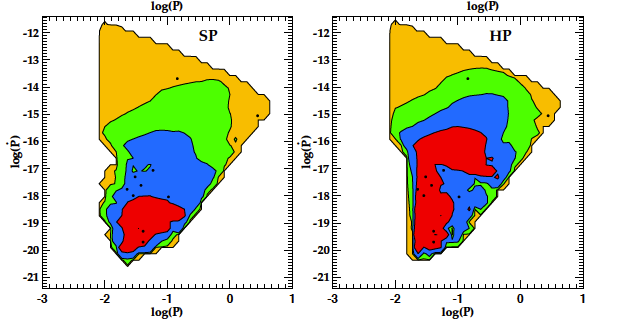
\includegraphics[scale=0.75]{intro/PopSynth.png}
%\caption{Courtesy of~\cite{OslowskiEtAl2011}. Shows the $P-\dot{P}$ distribution for two possible models.}
%\end{figure}
%\end{centering}

%Although these plots are not an exact representation of the actual binary population, as radio observation effects are taken into account, the takeaway is that there are models which can produce a large number of pulsars with $P\sim 10ms$, and $\dot{P}\sim 10^{-19}-10^{-20}$. With $\dot{P}$ that low, the pulsar would essentially have the same spin if it merged in 1Gyr or so. Furthermore, these models match up well on the $P-\dot{P}$ diagram with the known binary population. It appears that the hard edge on the low period side of the graphs is an artifact of the selection of all pulsars starting at $10ms$ - perhaps a more realistically modelled distribution would allow for even lower spin pulsars. Although these models are ultimately disfavoured to another model without as many low $\dot{P}$ pulsars by a further comparison to the chip mass distribution of known systems, based on all the free parameters and uncertainty involved in the study it seems reasonable to think that these models are physically plausible.

%\subsection{Hypercritical Accretion}
%We'll say a brief word on hypercritical accretion. During the common envelope phase, it is possible for super-Eddington accretion to be powered by neutrino losses. Although this process has been studied in the literature (see \cite{Chevalier1996} for example), the physical processes involved are quite complicated and uncertain. In is unclear whether or not this is a viable mechanism to produce millisecond pulsars, or whether black hole formation is inevitable due to the high mass gain. However, this is at least a plausible to produce highly spinning stars in neutron star binaries, and thus provides further motivation to study them.

%\section{Contemporary Research}
%\label{sec_PrevWork}
%Although as mentioned betore, corotation is an unphysical assumption, studies which have compared corotational configurations to irrotational configurations can still give us insight into the effects that highly spinning neutron stars can have on the dynamics of the system. We now review several studies that have done such comparisons.

%Shibata and Uryu (1999)\cite{ShibataUryu2000} simulated equal-mass mergers, with a $\Gamma=2$ equation of state using quasi-equilibrium initial data sequences starting very close to the merger. There was an extremely large difference found in the disk mass: For corotational configurations, a disk of mass $0.05-0.1M_{\odot}$ can be formed, whereas for irrotational configurations, the disk mass was $< 0.01M_{\odot}$. The merger remnant for two comparable configurations is shown in figure 3.

%\begin{centering}
%\begin{figure}[!ht]
%\label{fig_Shibata}
%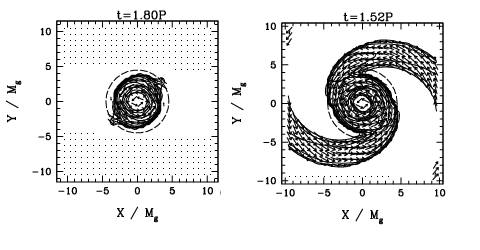
\includegraphics[scale=0.75]{intro/ShibataUryu.png}
%\caption{Courtsey of \cite{ShibataUryu2000}. A comparison of the disks formed from irrotational and corotational configurations.}
%\end{figure}
%\end{centering}

%Faber and Rasio (2000)\cite{FaberRasio2000} compared corotational and irrotational configurations using a Post-Newtonian SPH code. The results are qualitatively similar to Shibata and Uryu: corotation leads to a much more prominent disk.

%Duez et. al. (2002)\cite{DuezEtAl2002} focused on the inspiral phase, and the effect of corotation versus irrotation on the gravitational waveform. The result, simply stated, is that the amplitude of the waveform is the same at a given separation, but the corotational inspirals proceeds much quicker - It took the irrotational configuration 96.6 wave cycles to go from $r=10.8M$ to $r=6.78M$ compared to 62.1 cycles to go from $r=10.8M$ to $r=6.75M$ for the corotational configuration.

%Oechslin et. al. (2007)\cite{OechslinEtAl2007} used an SPH code which uses the conformal flatness approximation to general relativity. Interestingly, not only did they use corotational configurations with aligned spins, but also anti-aligned, oppositely aligned, and tilted spin configurations. The qualitative results are, again, that corotation leads to a much larger disk than irrotation ($0.21M_{\odot}$ compared to $0.04M_{\odot}$) for the Shen equation of state. Also, it is found that counterrotation severely suppresses the disk, and that tilted configurations have disk sizes similar to the aligned case.
